\documentclass[
11pt, % The default document font size, options: 10pt, 11pt, 12pt
%oneside, % Two side (alternating margins) for binding by default, uncomment to switch to one side
english,% ngerman for German
singlespacing, % Single line spacing, alternatives: onehalfspacing or doublespacing
%draft, % Uncomment to enable draft mode (no pictures, no links, overfull hboxes indicated)
%nolistspacing, % If the document is onehalfspacing or doublespacing, uncomment this to set spacing in lists to single
%liststotoc, % Uncomment to add the list of figures/tables/etc to the table of contents
%toctotoc, % Uncomment to add the main table of contents to the table of contents
parskip, % Uncomment to add space between paragraphs
%nohyperref, % Uncomment to not load the hyperref package
headsepline, % Uncomment to get a line under the header
%chapterinoneline, % Uncomment to place the chapter title next to the number on one line
%consistentlayout, % Uncomment to change the layout of the declaration, abstract and acknowledgements pages to match the default layout
]{MastersDoctoralThesis} % The class file specifying the document structure

\usepackage[utf8]{vietnam} % Required for inputting international characters
\graphicspath{{images/}}

%\usepackage{mathpazo} % Use the Palatino font by default

\usepackage[style=numeric,sorting=none,backend=bibtex,natbib=true]{biblatex} % Use the bibtex backend with the authoryear citation style (which resembles APA)
\usepackage{listings}
\bibliography{example.bib} % The filename of the bibliography

\usepackage[autostyle=true]{csquotes} % Required to generate language-dependent quotes in the bibliography

\usepackage{float}

\usepackage{listings}
\usepackage{color} % tô màu cho code
\definecolor{dkgreen}{rgb}{0,0.6,0}
\definecolor{gray}{rgb}{0.5,0.5,0.5}
\definecolor{mauve}{rgb}{0.58,0,0.82}
 
\lstset{frame=tb,
  language=Java,
  aboveskip=3mm,
  belowskip=3mm,
  showstringspaces=false,
  columns=flexible,
  basicstyle={\small\ttfamily},
  numbers=none,
  numberstyle=\tiny\color{gray},
  keywordstyle=\color{black},
  commentstyle=\color{dkgreen},
  stringstyle=\color{black},
  breaklines=true,
  breakatwhitespace=true,
  tabsize=4
}

%----------------------------------------------------------------------------------------
%	MARGIN SETTINGS
%----------------------------------------------------------------------------------------

\geometry{
	paper=a4paper, % Change to letterpaper for US letter
	inner=2.7cm, % Inner margin
	outer=2.7cm, % Outer margin
	%bindingoffset=.5cm, % Binding offset
	top=2cm, % Top margin
	bottom=2cm, % Bottom margin
	%showframe, % Uncomment to show how the type block is set on the page
}

%----------------------------------------------------------------------------------------
%	THESIS INFORMATION
%----------------------------------------------------------------------------------------

\thesistitle{DỰ ĐOÁN TÌNH TRẠNG GIAO THÔNG Ở THÀNH PHỐ HỒ CHÍ MINH} % Your thesis title, this is used in the title and abstract, print it elsewhere with \ttitle
\supervisor{TS. Trần Minh Quang} % Your supervisor's name, this is used in the title page, print it elsewhere with \supname
%\examiner{} % Your examiner's name, this is not currently used anywhere in the template, print it elsewhere with \examname
%\degree{Doctor of Philosophy} % Your degree name, this is used in the title page and abstract, print it elsewhere with \degreename
\author{Lê Công Huy\\ Nguyễn Hoàng Mẫn Tiến} % Your name, this is used in the title page and abstract, print it elsewhere with \authorname
%\addresses{} % Your address, this is not currently used anywhere in the template, print it elsewhere with \addressname

%\subject{Biological Sciences} % Your subject area, this is not currently used anywhere in the template, print it elsewhere with \subjectname
\keywords{} % Keywords for your thesis, this is not currently used anywhere in the template, print it elsewhere with \keywordnames
\university{\href{http://www.hcmut.edu.vn}{Trường Đại học Bách Khoa TP.HCM}} % Your university's name and URL, this is used in the title page and abstract, print it elsewhere with \univname
\department{\href{http://www.cse.hcmut.edu.vn}{Khoa Khoa học và Kỹ thuật Máy tính}} % Your department's name and URL, this is used in the title page and abstract, print it elsewhere with \deptname
%\group{\href{http://researchgroup.university.com}{Research Group Name}} % Your research group's name and URL, this is used in the title page, print it elsewhere with \groupname
%\faculty{\href{http://faculty.university.com}{Faculty Name}} % Your faculty's name and URL, this is used in the title page and abstract, print it elsewhere with \facname

\AtBeginDocument{
\hypersetup{linkcolor=black}
\hypersetup{urlcolor=black}
\hypersetup{citecolor=blue}
\hypersetup{pdftitle=\ttitle} % Set the PDF's title to your title
\hypersetup{pdfauthor=\authorname} % Set the PDF's author to your name
\hypersetup{pdfkeywords=\keywordnames} % Set the PDF's keywords to your keywords
}
\begin{document}

\frontmatter % Use roman page numbering style (i, ii, iii, iv...) for the pre-content pages

\pagestyle{plain} % Default to the plain heading style until the thesis style is called for the body content

%----------------------------------------------------------------------------------------
%	TITLE PAGE
%----------------------------------------------------------------------------------------

\begin{titlepage}
\begin{center}
{\scshape\Large \univname\par}{\large \deptname}\\% University name

\includegraphics[scale = 0.3]{logo.png}\\ \vspace{1.5cm}	% University Logo
\textsc{\LARGE Đề cương Luận văn}\\[0.5cm] % Thesis type

\hrulefill \\[0.4cm] % Horizontal line
{\huge \bfseries \ttitle\par}\vspace{0.4cm} % Thesis title
\hrulefill \\[1.5cm] % Horizontal line
 
\begin{minipage}[t]{0.4\textwidth}
\begin{flushleft} \large
\emph{Sinh viên:}\\
{\authorname} % Author name - remove the \href bracket to remove the link
\end{flushleft}
\end{minipage}
\begin{minipage}[t]{0.4\textwidth}
\begin{flushright} \large
\emph{GVHD:} \\
{\supname} % Supervisor name - remove the \href bracket to remove the link  
\end{flushright}
\end{minipage}\\[4cm]
 
\vfill

%\large \textit{A thesis submitted in fulfillment of the requirements\\ for the degree of \degreename}\\[0.3cm] % University requirement text
%\textit{in the}\\[0.4cm]
%\groupname\\\deptname\\[2cm] % Research group name and department name
 
\vfill

- { \large \today} -% Date
%\includegraphics{Logo} % University/department logo - uncomment to place it
 
\vfill
\end{center}
\end{titlepage}

\chapter{Lời cam đoan}
Chúng tôi cam đoan rằng, ngoại trừ các kết quả tham khảo từ các công trình nghiên cứu khoa học khác đã ghi rõ trong phần tài liệu tham khảo, tất cả những nội dung được trình bày trong luận văn này là do chính nhóm chúng tôi thực hiện và chưa có phần nội dung nào trong luận văn này được nộp để lấy bằng cấp ở một trường khác. Nếu có bất kỳ sai phạm nào, chúng tôi sẽ chịu hoàn toàn trách nhiệm trước Ban Chủ Nhiệm Khoa và Ban Giám Hiệu Nhà Trường.\\[1cm]

\begin{minipage}[t]{0.4\textwidth}
\hspace*{1cm}
\end{minipage}
\begin{minipage}[t]{0.6\textwidth}
\begin{center}
Thành phố Hồ Chí Minh, \today\\
\textbf{Nhóm nghiên cứu}
\end{center}
\end{minipage}

\chapter{Lời cảm ơn}
Lời nói đầu, chúng tôi xin được gửi lời cảm ơn chân thành và sâu sắc đến thầy giảng viên hướng dẫn TS. Trần Minh Quang đã hỗ trợ và có những đóng góp hết sức quý báu để giúp chúng tôi hoàn thành đề tài luận văn một cách tốt nhất. Trong suốt chặng đường nghiên cứu đề cương luận văn, thầy luôn là người định hướng và đề xuất những kiến thức mới mẻ về mặt khoa học cho đề tài.
Bên cạnh đó, chúng tôi cũng muốn thay mặt cho toàn thể sinh viên gửi lời biết ơn đến với quý thầy cô của trường Đại học Bách Khoa TPHCM nói chung, và của Khoa Khoa học và Kỹ thuật Máy Tính nói riêng vì công sức dạy dỗ tận tình và truyền tải nguồn tri thức vô giá cho nhóm nghiên cứu trong việc thực hiện đề tài đề cương luận văn cũng như trong con đường sự nghiệp sau này.

Xin chân thành cảm ơn.

Trân trọng.\\[1cm]

\begin{minipage}[t]{0.4\textwidth}
\hspace*{1cm}
\end{minipage}
\begin{minipage}[t]{0.6\textwidth}
\begin{center}
Thành phố Hồ Chí Minh, \today\\
\textbf{Nhóm nghiên cứu}
\end{center}
\end{minipage}


\chapter{Tóm tắt nội dung}
Đây là đề tài đề cương luận văn nghiên cứu về việc thu thập dữ liệu giao thông từ nhiều nguồn như Smart BK Traffic, Crowdsourcing nhằm đem lại nguồn dữ liệu đầy đủ, có độ chính xác cao hơn. Đồng thời áp dụng các phương pháp Data Mining để dự đoán và hiển thị tình trạng giao thông trên ứng dụng web.

Nội dung đề cương luận văn gồm có 8 chương:
\begin{itemize}
\item \textbf{Chương 1:} Giới thiệu.
\item \textbf{Chương 2:} Các nghiên cứu liên quan.
\item \textbf{Chương 3:} Các nguồn chia sẻ dữ liệu.
\item \textbf{Chương 4:} Kỹ thuật thu thập dữ liệu.
\item \textbf{Chương 5:} Thiết kế cơ sở dữ liệu.
\item \textbf{Chương 6:} Thiết kế hệ thống.
\item \textbf{Chương 7:} Đánh giá.
\item \textbf{Chương 8:} Kết luận và hướng phát triển.
\end{itemize}


%----------------------------------------------------------------------------------------
%	LIST OF CONTENTS/FIGURES/TABLES PAGES
%----------------------------------------------------------------------------------------


\tableofcontents % Prints the main table of contents

\listoffigures % Prints the list of figures

%\listoftables % Prints the list of tables


%
%%----------------------------------------------------------------------------------------
%%	ABBREVIATIONS
%%----------------------------------------------------------------------------------------
%
%\begin{abbreviations}{ll} % Include a list of abbreviations (a table of two columns)
%
%\textbf{LAH} & \textbf{L}ist \textbf{A}bbreviations \textbf{H}ere\\
%\textbf{WSF} & \textbf{W}hat (it) \textbf{S}tands \textbf{F}or\\
%
%\end{abbreviations}
%
%%----------------------------------------------------------------------------------------
%%	PHYSICAL CONSTANTS/OTHER DEFINITIONS
%%----------------------------------------------------------------------------------------
%
%\begin{constants}{lr@{${}={}$}l} % The list of physical constants is a three column table
%
%% The \SI{}{} command is provided by the siunitx package, see its documentation for instructions on how to use it
%
%Speed of Light & $c_{0}$ & \SI{2.99792458e8}{\meter\per\second} (exact)\\
%%Constant Name & $Symbol$ & $Constant Value$ with units\\
%
%\end{constants}
%
%%----------------------------------------------------------------------------------------
%%	SYMBOLS
%%----------------------------------------------------------------------------------------
%
%\begin{symbols}{lll} % Include a list of Symbols (a three column table)
%
%$a$ & distance & \si{\meter} \\
%$P$ & power & \si{\watt} (\si{\joule\per\second}) \\
%%Symbol & Name & Unit \\
%
%\addlinespace % Gap to separate the Roman symbols from the Greek
%
%$\omega$ & angular frequency & \si{\radian} \\
%
%\end{symbols}
%
%%----------------------------------------------------------------------------------------
%%	DEDICATION
%%----------------------------------------------------------------------------------------
%
%\dedicatory{For/Dedicated to/To my\ldots} 

%----------------------------------------------------------------------------------------
%	THESIS CONTENT - CHAPTERS
%----------------------------------------------------------------------------------------

\mainmatter % Begin numeric (1,2,3...) page numbering

\pagestyle{thesis} % Return the page headers back to the "thesis" style

% Include the chapters of the thesis as separate files from the Chapters folder
% Uncomment the lines as you write the chapters

% Chapter 1

\chapter{Giới thiệu} % Main chapter title

\label{Chapter1} % For referencing the chapter elsewhere, use \ref{Chapter1} 

%----------------------------------------------------------------------------------------

% Define some commands to keep the formatting separated from the content 
\newcommand{\keyword}[1]{\textbf{#1}}
\newcommand{\tabhead}[1]{\textbf{#1}}
\newcommand{\code}[1]{\texttt{#1}}
\newcommand{\file}[1]{\texttt{\bfseries#1}}
\newcommand{\option}[1]{\texttt{\itshape#1}}

%----------------------------------------------------------------------------------------

\section{Tổng quan}
\section{Nhiệm vụ đề cương luận văn}

% Chapter 2

\chapter{Các nghiên cứu liên quan} % Main chapter title

\label{Chapter2} % For referencing the chapter elsewhere, use \ref{Chapter1} 

Trước tình hình giao thông ngày càng đông đúc và dày đặc tại các thành phố lớn, trong đó có thành phố Hồ Chí Minh, nhiều biện pháp, nghiên cứu cũng được đề ra để giải quyết vấn đề nhức nhối này \cite{FSPPM}. Tuy nhiên, phần lớn các báo cáo khoa học hay nghiên cứu đều tập trung vào cách thu thập dữ liệu và đưa ra dự đoán 

Phần lớn các báo cáo khoa học hay nghiên cứu chủ yếu tập trung vào cách thu thập dữ liệu (data collection method) về luồng giao thông (traffic flow) nhằm phân tích và đưa ra dự đoán bằng những thiết bị cảm biến, radar, sóng âm hay nhận diện bằng hình ảnh, video hay thậm chí ước lượng thủ công (manual count) [10] [11]. Các phương pháp này đều cần một hệ thống cơ sở hạ tầng hiện đại, tiên tiến để thu thập dữ liệu và phân tích sau đó đưa ra kết quả nhằm mục đích nghiên cứu lâu dài.

Sở giao thông thành phố Hồ Chí Minh cũng đã có đưa ra ứng dụng [12] [13] cho phép người dân có thể xem tình trạng giao thông từ các camera đặt tại các ngã 4, ngã 3 tại thời điểm hiện tại, thông báo về hiện trạng giao thông tại các tuyến đường qua các màn hình lớn trên đường. Hệ thống này còn thu thập dữ liệu từ GPS của các tuyến xe buýt để đưa ra những đánh giá về tốc độ có thể di chuyển được trên những tuyến đường. Đại học Bách Khoa thành phố Hồ Chí Minh cũng có một nhóm nghiên cứu hiện thực một trang web thông báo tình trạng giao thông từ GPS của các tuyến xe bus [13] tương tự như hệ thống trên. Tuy nhiên những hệ thống này đều dựa vào các thiết bị định vị GPS hay các hệ thống cảm biến cố định (fixed sensor). Từ năm 2014 đến giữa năm 2018, số lượng người sử dụng thiết bị điện thoại thông minh gia tăng rất nhanh (hình
2.1) đã đưa ra một hướng thu thập dữ thiệu khác từ chính những chiếc điện thoại thông minh này.

Sự phát triển của các thiết bị di động đã tạo điều kiện cho một hướng thu thập dữ liệu khác đó là từ cộng đồng, hay còn gọi là thu thập dữ liệu cộng đồng (crowdsourcing). Có thể hiểu crowsourcing như là một tổ chức, một công ty hay một cá nhân nào đó nhằm thu thập dữ liệu, thông tin để hoàn thành một nhiệm vụ nào đó từ cộng đồng [14] [15]. Sau khi nhận được yêu cầu, cộng đồng này sẽ đưa ra giải pháp, cung cấp dữ liệu cho người yêu cầu để hoàn thành mục đích của họ. Đổi lại, cộng đồng này sẽ nhận được những phần thưởng tương xứng như tiền, danh tiếng (reputation) trong cộng đồng, sự tôn trọng từ những người trong cộng đồng, quyền xem các dữ liệu hay thông tin do những người khác từ cộng đồng chia sẻ và sự thỏa mãn khi cảm thấy mình có đóng góp giúp ích cho xã hội.

Việc sử dụng nguồn lực cộng đồng (crowdsourcing) để thu thập dữ liệu hiện đang được các tổ chức, công ty [16] tích hợp vào các hệ thống hỏi đáp, truy xuất thông tin như Wikipedia, Yahoo! Answer, Youtube, Stackoverflow..., và trong các thảm họa thiên tai trong khoảng 10 năm trở lại đây [17] [18] [19] [20] [21] [22]. Các trang mạng xã hội như Facebook, Twitter... hiện nay để có một tính năng thông báo về sự an toàn của bản thân trong các tình huống xảy ra thảm họa thiên tai. Vào năm 2010, trong trận động đất ở Haiti, hệ thống Ushahidi đã hoạt động rất hiệu quả trong việc thu thập dữ liệu, phân tích và đưa ra những chỉ dẫn trực tiếp cho các tình nguyện viên để sơ tán, di tản người dân Haiti về khu vực an toàn [23] [24].

Tuy việc áp dụng những cảnh báo từ cộng đồng nhằm thu thập các thông tin về tình trạng giao thông đã xuất hiện nhưng việc xác thực dữ liệu (data validity) vẫn chưa thật sự được chú trọng mặc dù đây là một phần vô cùng quan trọng nhằm xác định độ chính xác của dữ liệu cũng như để phân tích và đưa ra những dự đoán. Do đó, nhóm nghiên cứu đã đưa ra giải pháp nhằm giải quyết bài toàn này. Bên cạnh đó, các dữ liệu sau khi được chia sẻ bởi cộng đồng cũng được nghiên cứu để thực hiện việc gom cụm (cluster) nhằm đem đến do cộng đồng một cái nhìn đơn giản, dễ hình dung hơn về tình trạng giao thông trên bản đồ của thành phố Hồ Chí Minh. Việc nghiên cứu này đã được hiện thực bằng một phiên bản ứng dụng di động trên nền tảng Android và iOS để tiếp tục tiến hành
việc kiểm tra tính hiệu quả của quá trình nghiên cứu. 
% Chapter 3

\chapter{Các nguồn chia sẻ dữ liệu} % Main chapter title

\label{Chapter3}

\section{HERE Real-time Traffic}
HERE Real-time Traffic là một dịch vụ của HERE Technologies - một công ty nổi tiếng và có kinh nghiệm trong việc cung cấp các dịch vụ về bản đồ và vị trí. Dịch vụ trên giúp người dùng có thể xác định vị trí, thời gian và lý do tắc nghẽn giao thông xảy ra bằng cách cung cấp tình trạng giao thông và các sự cố từng phút. Nguồn dữ liệu của dịch vụ được cung cấp và phân tích từ nhiều nguồn tổng hợp như cảm biến của ôtô, các cảm biến cố định trên đường hoặc từ các thiết bị sử dụng các ứng dụng của công ty. Năm 2017, HERE thông báo dịch vụ HERE Real-time Traffic cũng đã hỗ trợ ở Việt Nam.\cite{HERE}

\begin{figure}[!ht]
	\begin{center}
		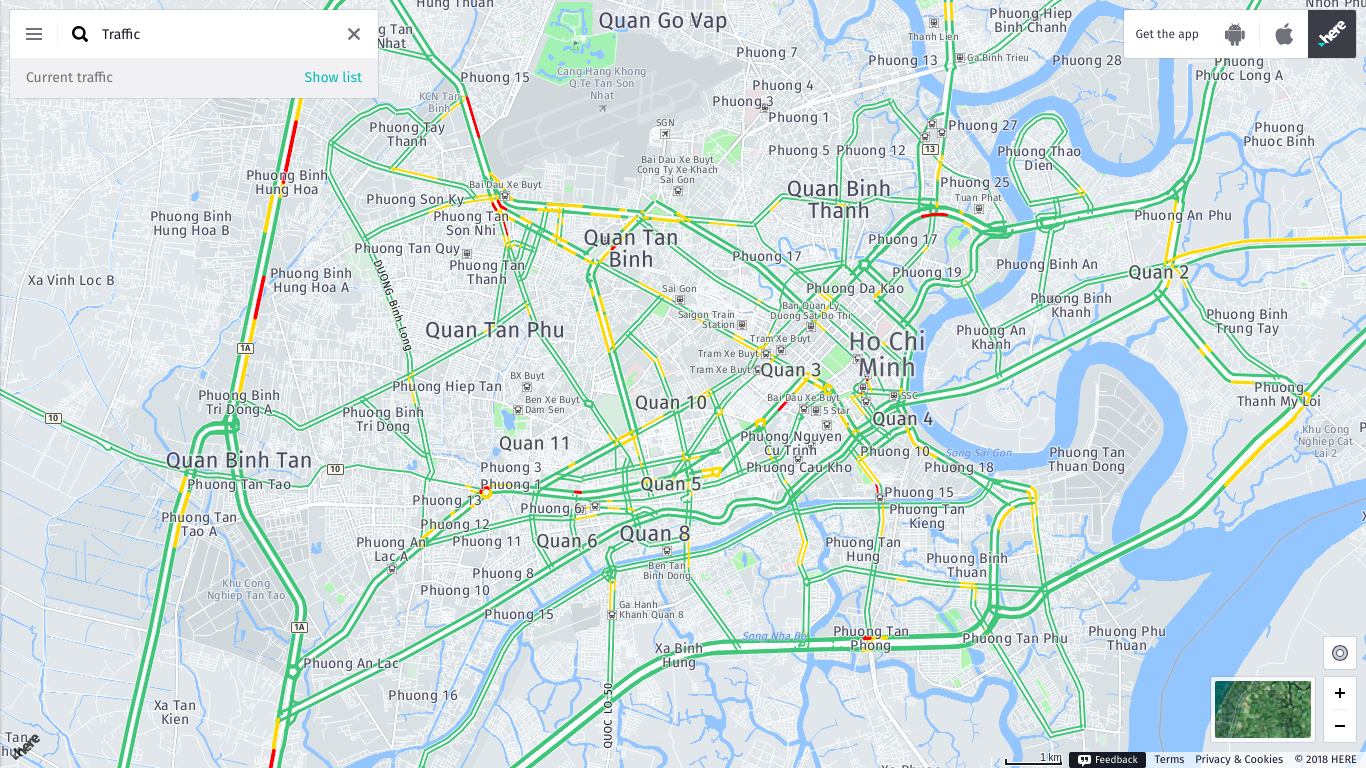
\includegraphics[width=1.0\textwidth]{images/here_maps.png}
	\end{center}
	\caption{HERE Real-time Traffic được sử dụng trên Here maps}
\end{figure}

Mặc dù được HERE giới thiệu rằng dịch vụ cung cấp nguồn dữ liệu thời gian thực và có độ chính xác cao. Tuy nhiên khi tiến hành tìm hiểu và nghiên cứu dịch vụ bằng cách sử dụng các API để lấy dữ liệu giao thông và so sánh với tình trạng giao thông ở một số thời điểm thực tế, nhóm nhận thấy dữ liệu dịch vụ cung cấp vẫn chưa thật sự có độ chính xác cao ở Việt Nam, cụ thể là thành phố Hồ Chí Minh. Vì thế, nhóm quyết định tạm dừng việc sử dụng HERE Real-time traffic lấy dữ liệu giao thông và tìm hiểu một số nguồn cung cấp dữ liệu khác.
\section{Smart BK Traffic}
Hệ thống giao thông thông minh (Smart BK Traffic) là hệ thống được nhóm Intelligent Transportation Systems Group (ITSG) tại trường Đại học Bách Khoa phát triển. Hệ thống được xây dựng để thu thập xử lý tín hiệu GPS từ xe hơi, xe taxi, xe buýt, thiết bị di động; đồng thời cung cấp dữ liệu đã được xử lý đến các ứng ụng web và điện thoại thông minh theo thời gian thực.

\begin{figure}[!ht]
	\begin{center}
		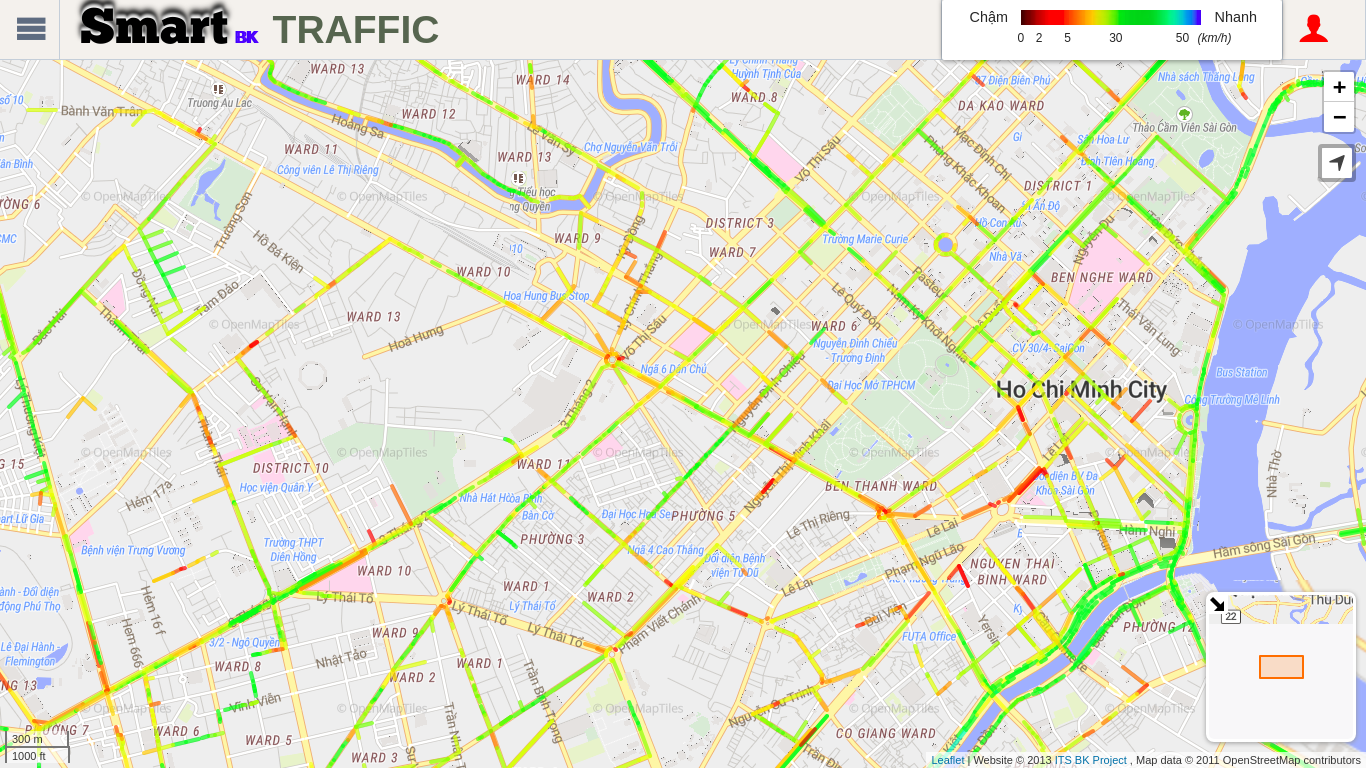
\includegraphics[width=1.0\textwidth]{images/smartbktraffic.png}
	\end{center}
	\caption{Website của hệ thống Smart BK Traffic - 17:45 08/12/2018}
\end{figure}

Sau một thời gian tìm hiểu và đánh giá, nhóm nhận thấy dữ liệu do hệ thống Smart BK Traffic cung cấp tương đối chính xác đối với tình trạng giao thông của thành phố Hồ Chí Minh. Mặc dù dữ liệu vẫn bị thiếu ở một số tuyến đường nhưng nhìn chung vẫn khá đầy đủ. Do đó, nhóm quyết định sử dụng nguồn dữ liệu này, kết hợp với nguồn dữ liệu crowdsourcing để có thể khai phá, đưa ra dự đoán tình hình giao thông ở những đoạn đường bị thiếu nhằm bổ sung vào những thiếu sót mà hệ thống đang có. Chi tiết về cách thu thập cũng như sử dụng dữ liệu sẽ được nhóm trình bày vào phần 4.
\section{Dữ liệu từ cộng đồng (Crowdsourcing)}
Như đã trình bày ở trên, nguồn dữ liệu thu thập được từ cộng đồng là một nguồn dữ liệu quan trọng và không thể thiếu trong quá trình làm đề tài. Một ví dụ cho tính hiệu quả của việc sử dụng nguồn dữ liệu cộng đồng ở Việt Nam là hệ thống VOV Giao thông 91Mhz của Đài tiếng nói Việt Nam, với cách thức thông báo tình trạng giao thông thông qua sóng radio với nguồn thông tin chính xác đến từ các tài xế lái xe, từ đó giúp cho các tài xế khác có thể điều chỉnh lộ trình của mình cho phù hợp, tránh đi những tuyến đường bị kẹt xe. Tuy nhiên việc sử dụng dữ liệu cộng đồng như thế vẫn còn rất nhiều hạn chế, cho nên cần một giải pháp khác để khai thác, sử dụng hiệu quả nguồn dữ liệu từ cộng đồng hơn. Cụ thể, nhóm kết hợp với hai nhóm khác cũng làm đề tài liên quan đến giao thông để xây dựng hệ thống cung cấp thông tin giao thông theo thời gian thực cho người dùng thông qua ứng dụng di động, với nguồn dữ liệu đến từ chính cộng đồng người dùng của ứng dụng.

Nhóm sẽ trình bày chi tiết và cụ thể hơn về kỹ thuật thu thập dữ liệu bằng các nguồn dữ liệu ở phần tiếp theo.

% Chapter 4

\chapter{Kỹ thuật thu thập dữ liệu} % Main chapter title

\label{Chapter4}
\section{Smart BK Traffic}
Sau quá trình tìm hiểu ngắn, nhóm nhận thấy hệ thống Smart BK Traffic cung cấp một số API để có thể lấy được dữ liệu về tình trạng giao thông thành phố Hồ Chí Minh tại thời điểm sử dụng. Trong đó, API quan trọng nhất được nhóm sử dụng là:
\begin{itemize}
    \item \textit{https://traffic.hcmut.edu.vn/hcm/rest/tc/init?} với các tham số truyền vào là tọa độ của 4 góc bản đồ cần lấy dữ liệu và độ zoom của map, cụ thể là:
\begin{itemize}
    \item latTL, lonTL: vĩ độ, kinh độ của điểm góc trên cùng bên trái
    \item latTR, lonTR: vĩ độ, kinh độ của điểm góc trên cùng bên phải
    \item latBL, lonBL: vĩ độ, kinh độ của điểm góc dưới cùng bên trái
    \item latBR, lonBR: vĩ độ, kinh độ của điểm góc dưới cùng bên phải
    \item zoom: độ zoom của bản đồ
\end{itemize}
    API trên trả về dữ liệu giao thông ở thời điểm gọi API và có cấu trúc như sau:
\begin{lstlisting}[language=XML]
{
  "segs": [
    {
      "v": "lat1,lon1,lat2,lon2,velocity,description,accuracy,id"
    }
  ],
  "last": boolean,
  "key": "key"
}
\end{lstlisting}
    Trong đó:
    \begin{itemize}
        \item "segs": là một mảng các segment, thông tin mỗi segment được lưu trong field "v" với các thuộc tính được phân cách nhau bằng dấu phẩy:
        \begin{itemize}
            \item lat1,lon1: vĩ độ, kinh độ điểm đầu của segment
            \item lat2,lon2: vĩ độ, kinh độ điểm cuối của segment
            \item velocity: vận tốc trên đoạn segment đó 
            \item description: miêu tả về đoạn segment
            \item accuracy: độ chính xác của giá trị vận tốc
            \item id: id của field "v".
        \end{itemize}
    
    \item "last": có giá trị boolean để xác định segment trả về đã là cuối cùng hay chưa. Nếu chưa thì sẽ có giá trị bằng \textit{false} và tạo ra key ở field "key" để có thể tiếp tục get dữ liệu.
    \item "key": tham số của API \textit{https://traffic.hcmut.edu.vn/hcm/rest/?key=} để get tiếp dữ liệu các segment còn thiếu.
    \end{itemize}
\end{itemize}
Sau khi đã hiểu rõ được cách làm việc của API, nhóm viết một chương trình nhỏ chạy trên server để lấy dữ liệu toàn thành phố Hồ Chí Minh mỗi 15 phút và lưu xuống database Mongodb.

Để lấy được dữ liệu của toàn thành phố, nhóm xác định bốn điểm tọa độ của vùng bao phủ thành phố và từ đó chia nhỏ ra thành 16x16 vùng nhỏ hơn để có thể thu thập dữ liệu được chính xác hơn. Vì nếu chỉ sử dụng bốn điểm tọa độ của vùng bao phủ thành phố thì API chỉ trả về dữ liệu của một số tuyến đường quan trọng trên bản đồ, dẫn đến sự thiếu sót dữ liệu. Sau khi xác định được các vùng nhỏ để tránh sự thiếu sót dữ liệu, nhóm sử dụng các API trình bày ở trên để thu thập và lưu dữ liệu theo cấu trúc của các model mà nhóm đã thảo luận, thống nhất với hai nhóm làm đề tài giao thông khác. Chi tiết về thiết kế cơ sở dữ liệu sẽ được trình bày ở phần 5.

\section{Dữ liệu từ cộng đồng (Crowdsourcing)}
Ở giai đoạn đề cương luận văn, việc thu thập dữ liệu từ cộng đồng chỉ dừng lại ở những bước xây dựng nền tảng để có thể thực hiện thu thập dữ liệu ở giai đoạn sau. Do đó, nhóm tham gia thảo luận với hai nhóm làm đề tài giao thông còn lại và đưa ra các đánh giá, nhận xét để xây dựng mô hình quan hệ thực thể, cấu trúc dữ liệu, thảo luận các phương pháp đánh giá tính xác thực của dữ liệu. Về việc xây dựng ứng dụng di động để thu thập dữ liệu từ cộng đồng, nhóm chỉ tham gia hỗ trợ chứ không trực tiếp xây dựng nên ở phạm vi đề cương luận văn này, nhóm chỉ trình bày sơ lược cách thu thập dữ liệu từ cộng đồng thông qua ứng dụng.

Cụ thể, sau khi người dùng cài đặt ứng dụng, người dùng có thể gửi những báo cáo liên quan đến tình trạng giao thông ở đoạn đường xảy ra kẹt xe. Báo cáo sẽ bao gồm các thông tin như thông tin đoạn đường, vận tốc hiện tại của đoạn đường, thời gian, mô tả, hình ảnh. Dữ liệu báo cáo sẽ được gửi lên server để lưu trữ cho việc phân tích, đồng thời gửi cảnh báo đến những người dùng khác về tình trạng giao thông ở đoạn đường đó. Từ đó, người dùng khác nếu ở gần sẽ có thể đánh giá độ chính xác của báo cáo đó. Để việc báo cáo được đơn giản hơn, ba nhóm cũng thảo luận, nghiên cứu đưa công nghệ speech to text áp dụng vào việc gửi báo cáo. Đồng thời, đưa ra các hình thức khuyến khích người dùng chia sẽ dữ liệu bằng hệ thống vinh danh, quà tặng.

 
% Chapter 1

\chapter{Thiết kế cơ sở dữ liệu} % Main chapter title

\label{Chapter5}

\section{Mô hình quan hệ thực thể} 
% Chapter 6

\chapter{Thiết kế hệ thống} % Main chapter title

\label{Chapter6}
\section{Tổng quan}
\section{Ứng dụng web (Front-end)}
\section{Server (Back-end)}
% Chapter 7

\chapter{Đánh giá} % Main chapter title

\label{Chapter7} 
% Chapter 8

\chapter{Kết luận và hướng phát triển} % Main chapter title

\label{Chapter8}

\section{Kết luận}
Với sự phát triển phức tạp của giao thông ở thành phố Hồ Chí Minh, tình hình ùn tắc giao thông ngày càng trở nên nghiêm trọng. Việc thu thập, phân tích và dự đoán tình trạng giao thông vì vậy mà trở nên rất cần thiết.

Qua giai đoạn đầu của quá trình nghiên cứu đề tài, nhóm đã thu được nhiều kết quả khả quan và một số hạn chế nhất định. Những kết quả đạt được và kinh nghiệm rút ra là bước chuẩn bị để thực hiện đề tài vào thời gian tới.

\section{Hướng phát triển}
Ở giai đoạn tiếp theo, nhóm sẽ tiếp tục phát triển đề tài theo cá mục tiêu:
\begin{itemize}
    \item Tiếp tục tìm hiểu và thu thập dữ liệu để có kết quả khách quan và chính xác hơn.
    \item Nghiên cứu các kỹ thuật Data Mining để tối ưu hoá độ chính xác khi dự đoán.
    \item Từ các dữ liệu đã thu thập được, thực hiện khai phá dữ liệu để dự đoán tình trạng giao thông, nhất là ở những đoạn đường chưa có dữ liệu trực tiếp.
    \item Hoàn thiện ứng dụng web và xây dựng thêm một số chức năng hỗ trợ người dùng.
\end{itemize} 

%----------------------------------------------------------------------------------------
%	THESIS CONTENT - APPENDICES
%----------------------------------------------------------------------------------------

\appendix % Cue to tell LaTeX that the following "chapters" are Appendices

% Include the appendices of the thesis as separate files from the Appendices folder
% Uncomment the lines as you write the Appendices

%% Appendix A

\chapter{Frequently Asked Questions} % Main appendix title

\label{AppendixA} % For referencing this appendix elsewhere, use \ref{AppendixA}

\section{How do I change the colors of links?}

The color of links can be changed to your liking using:

{\small\verb!\hypersetup{urlcolor=red}!}, or

{\small\verb!\hypersetup{citecolor=green}!}, or

{\small\verb!\hypersetup{allcolor=blue}!}.

\noindent If you want to completely hide the links, you can use:

{\small\verb!\hypersetup{allcolors=.}!}, or even better: 

{\small\verb!\hypersetup{hidelinks}!}.

\noindent If you want to have obvious links in the PDF but not the printed text, use:

{\small\verb!\hypersetup{colorlinks=false}!}.

%\include{Appendices/AppendixB}
%\include{Appendices/AppendixC}

%----------------------------------------------------------------------------------------
%	BIBLIOGRAPHY
%----------------------------------------------------------------------------------------

\printbibliography

%----------------------------------------------------------------------------------------

\end{document}  
